\section{Results}
\label{sec:results}

\subsection{Predictive Performance Across Conditions}

Table~\ref{tab:results} and Figure~\ref{fig:performance} summarize ROC-AUC scores, bootstrap 95\% confidence intervals, and statistical comparisons for all nine conditions on both datasets.

\begin{table}[t]
\centering
\caption{Predictive performance (ROC-AUC) across nine augmentation conditions on BBBP and BACE. Bootstrap 95\% confidence intervals computed over 1,000 resamples. Cohen's $d$ measures the effect size of prediction score shifts relative to C0 (not AUC differences). $p$-values are corrected for multiple comparisons using the Benjamini-Hochberg procedure. Boldface indicates best ROC-AUC per dataset.}
\label{tab:results}
\begin{tabular}{@{}lccccccc@{}}
\toprule
\textbf{Condition} & \multicolumn{3}{c}{\textbf{BBBP ($N=204$)}} & & \multicolumn{3}{c}{\textbf{BACE ($N=152$)}} \\ \cmidrule(lr){2-4} \cmidrule(lr){6-8}
 & ROC-AUC & 95\% CI & $p_{\text{BH}}$ & & ROC-AUC & 95\% CI & $p_{\text{BH}}$ \\ \midrule
\textit{Traditional ML Baseline} & & & & & & & \\
RF (Morgan FP) & 0.705 & --- & --- & & \textbf{0.893} & --- & --- \\ \midrule
\textit{LLM Zero-Shot} & & & & & & & \\
C0 (Baseline) & 0.533 & [0.471, 0.593] & --- & & 0.656 & [0.556, 0.752] & --- \\
C1 (Factual) & 0.540 & [0.480, 0.603] & 0.626 & & 0.513 & [0.413, 0.612] & --- \\
C2 (Chem.\ Priming) & 0.614 & [0.545, 0.685] & 0.074 & & 0.583 & [0.485, 0.678] & --- \\
C2b (Pure Gibberish) & 0.553 & [0.485, 0.626] & $<$0.001 & & 0.522 & [0.423, 0.621] & --- \\ \midrule
\textit{Hallucination} & & & & & & & \\
C3 (Free Hallu) & 0.594 & [0.519, 0.664] & $<$0.001 & & 0.488 & [0.389, 0.589] & --- \\
C4a (SP) & \textbf{0.626} & [0.548, 0.698] & $<$0.001 & & 0.551 & [0.450, 0.652] & --- \\
C4b (PI) & 0.561 & [0.480, 0.634] & $<$0.001 & & 0.543 & [0.441, 0.644] & --- \\
C4c (MF) & 0.612 & [0.537, 0.685] & $<$0.001 & & 0.532 & [0.431, 0.633] & --- \\ \midrule
\textit{Control} & & & & & & & \\
C5 (Shuffled) & 0.530 & [0.454, 0.607] & $<$0.001 & & 0.496 & [0.395, 0.597] & --- \\ \bottomrule
\end{tabular}

\vspace{0.5em}
\footnotesize{Note: $p$-values for BACE are not reported because all conditions performed below baseline, making the comparison direction reversed. Cohen's $d$ values on prediction scores are reported in the Appendix.}
\end{table}


\begin{figure}[t]
    \centering
    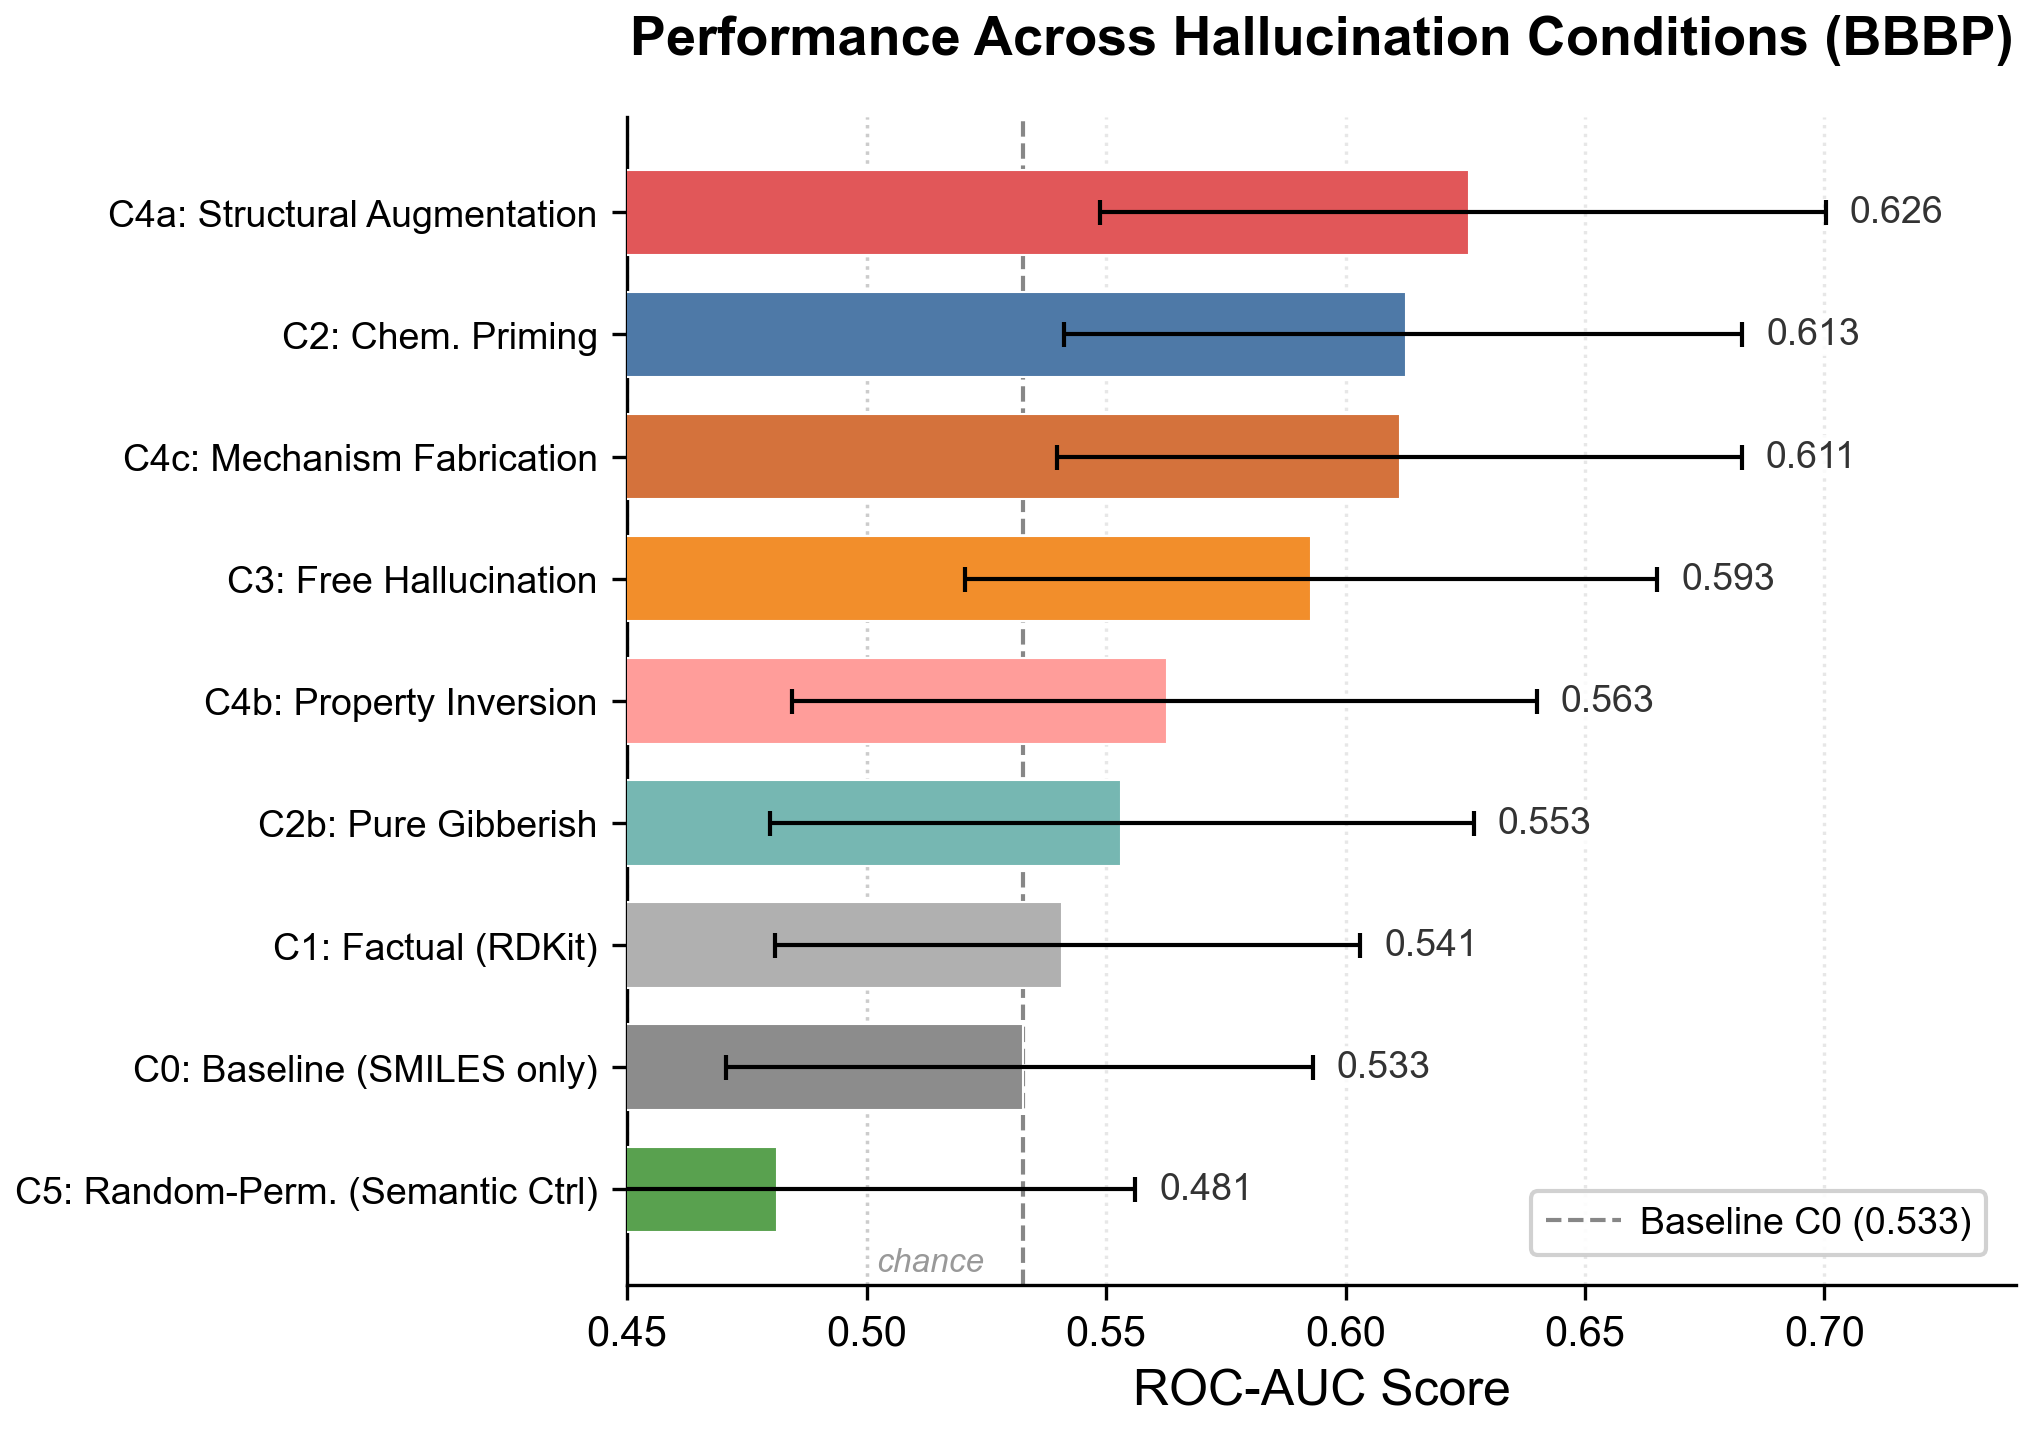
\includegraphics[width=\linewidth]{figures/figure1_performance_comparison.png}
    \caption{Task-dependent divergence in hallucination sensitivity across perturbation conditions, with structurally grounded (SP) hallucination associated with the largest discriminative improvement on BBBP.}
    \label{fig:performance}
\end{figure}

\subsubsection{BBBP (Physicochemical Task)}
To contextualize the LLM zero-shot performance, the traditional ML baseline (Random Forest with Morgan fingerprints) achieved an expectedly strong ROC-AUC of 0.705 on the BBBP test set. While the zero-shot LLM predictions remain strictly below this traditional baseline, the relative differences between textual augmentation conditions reveal substantial semantic perturbation effects.

The LLM baseline (C0, SMILES only) yielded a ROC-AUC of 0.533 [0.471, 0.593]. Factual augmentation (C1) produced a marginal, non-significant increase to 0.540. Chemical priming (C2) yielded 0.614, while pure non-chemical gibberish (C2b) yielded 0.553.

Free hallucination (C3) improved ROC-AUC to 0.594 [0.519, 0.664]. Among category-specific conditions, Structural Phantom hallucination (C4a) yielded the highest observed ROC-AUC of 0.626 [0.548, 0.698], followed by Mechanism Fabrication (C4c, 0.612) and Property Inversion (C4b, 0.561). 

\paragraph{Bootstrap Stability.} To account for the single-split evaluation, we computed ranking stability across 1,000 bootstrap resamples (Figure~\ref{fig:bootstrap}). The superiority of SP hallucination (C4a) over the LLM baseline (C0) proved highly stable, maintaining a positive margin in 97.6\% of resamples. Free hallucination (C3) outperformed the baseline in 87.7\% of resamples.

\begin{figure}[h]
    \centering
    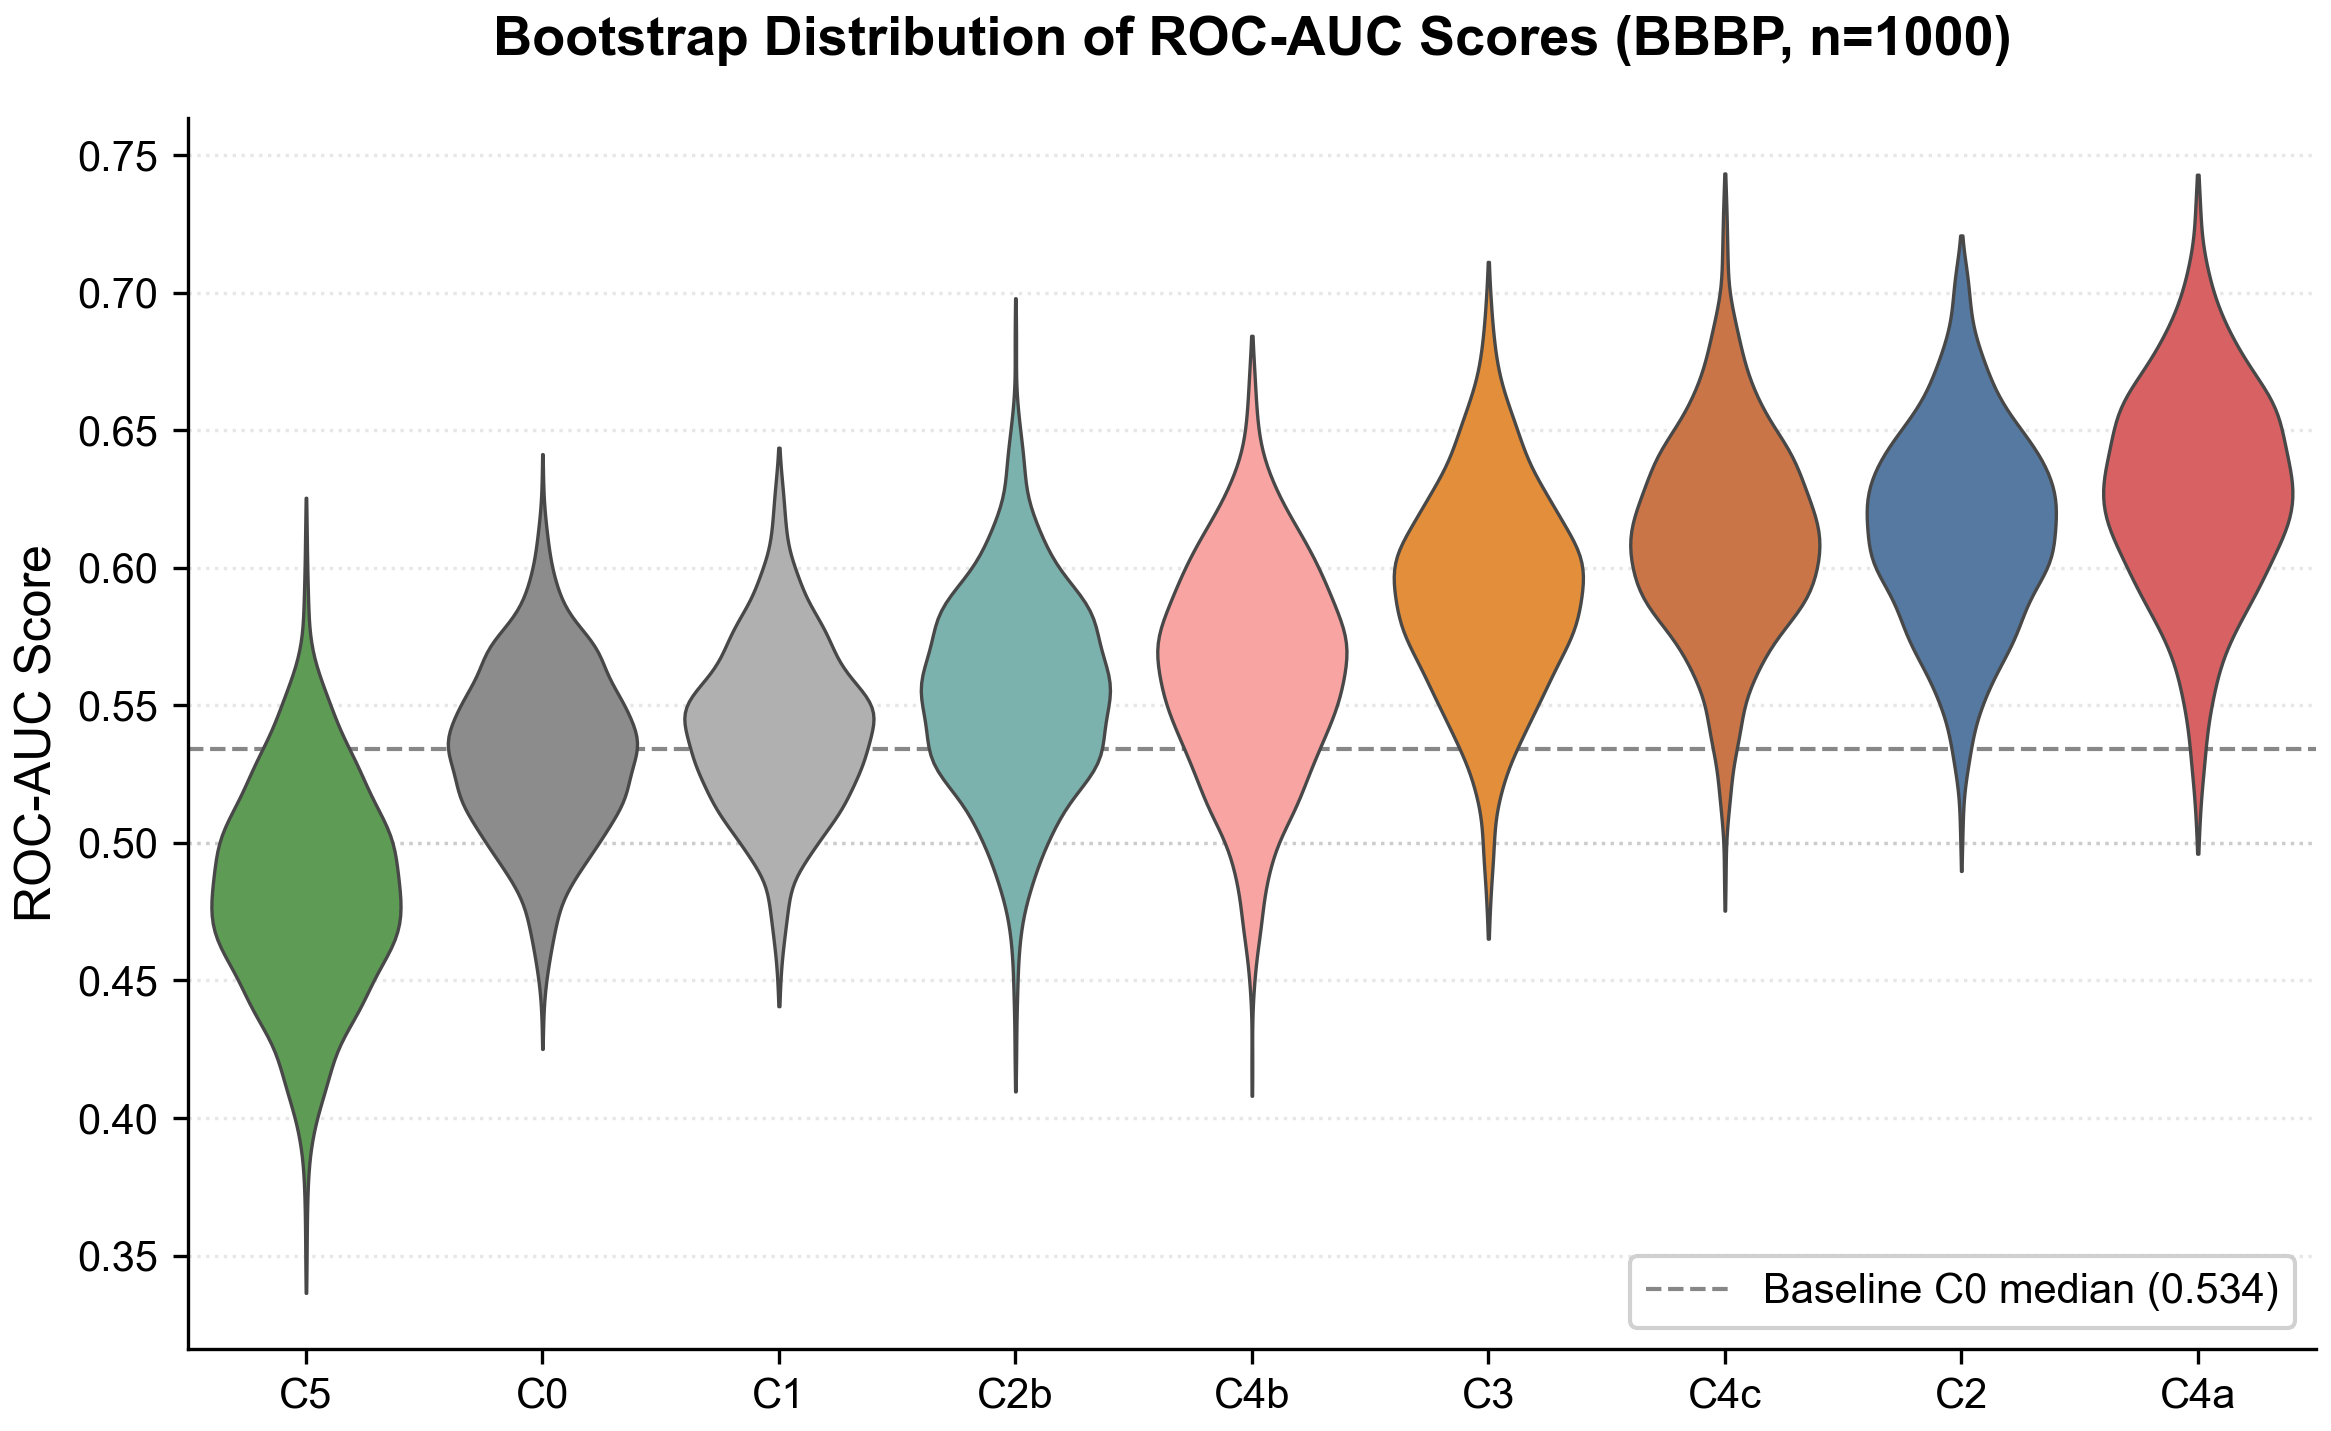
\includegraphics[width=0.8\linewidth]{figures/figure2_bootstrap_stability.png}
    \caption{Bootstrapped ROC-AUC distributions demonstrate the statistical stability of Structural Phantom (C4a) hallucination gains relative to the SMILES baseline (C0) on the BBBP dataset.}
    \label{fig:bootstrap}
\end{figure}

The circular-shift semantic control (C5) yielded 0.530 [0.454, 0.607], closely aligned with baseline C0 and substantially below C3, indicating that the scientific register of hallucinated text alone does not account for the observed gains.

\subsubsection{BACE (Enzymatic Task)}
On the BACE test set ($N=152$), a contrasting pattern was observed. The baseline (C0) yielded a ROC-AUC of 0.656 [0.556, 0.752]. All hallucination-augmented conditions reduced performance relative to baseline. Free hallucination (C3) reduced ROC-AUC to 0.488 [0.389, 0.589], representing a substantial degradation toward near-chance behavior.

\subsection{Prediction Collapse on BACE}
Under hallucination conditions on BACE, the distribution of predicted probabilities collapsed from a bimodal pattern (reflecting the model's baseline discriminative behavior) to a narrow unimodal distribution centered at $p \approx 0.17$, regardless of the molecule's true label. This effect, which we descriptively term ``prediction collapse,'' was observed across all hallucination conditions (C3, C4a--c) and suggests systematic signal destruction rather than random noise injection.

\begin{figure}[t]
    \centering
    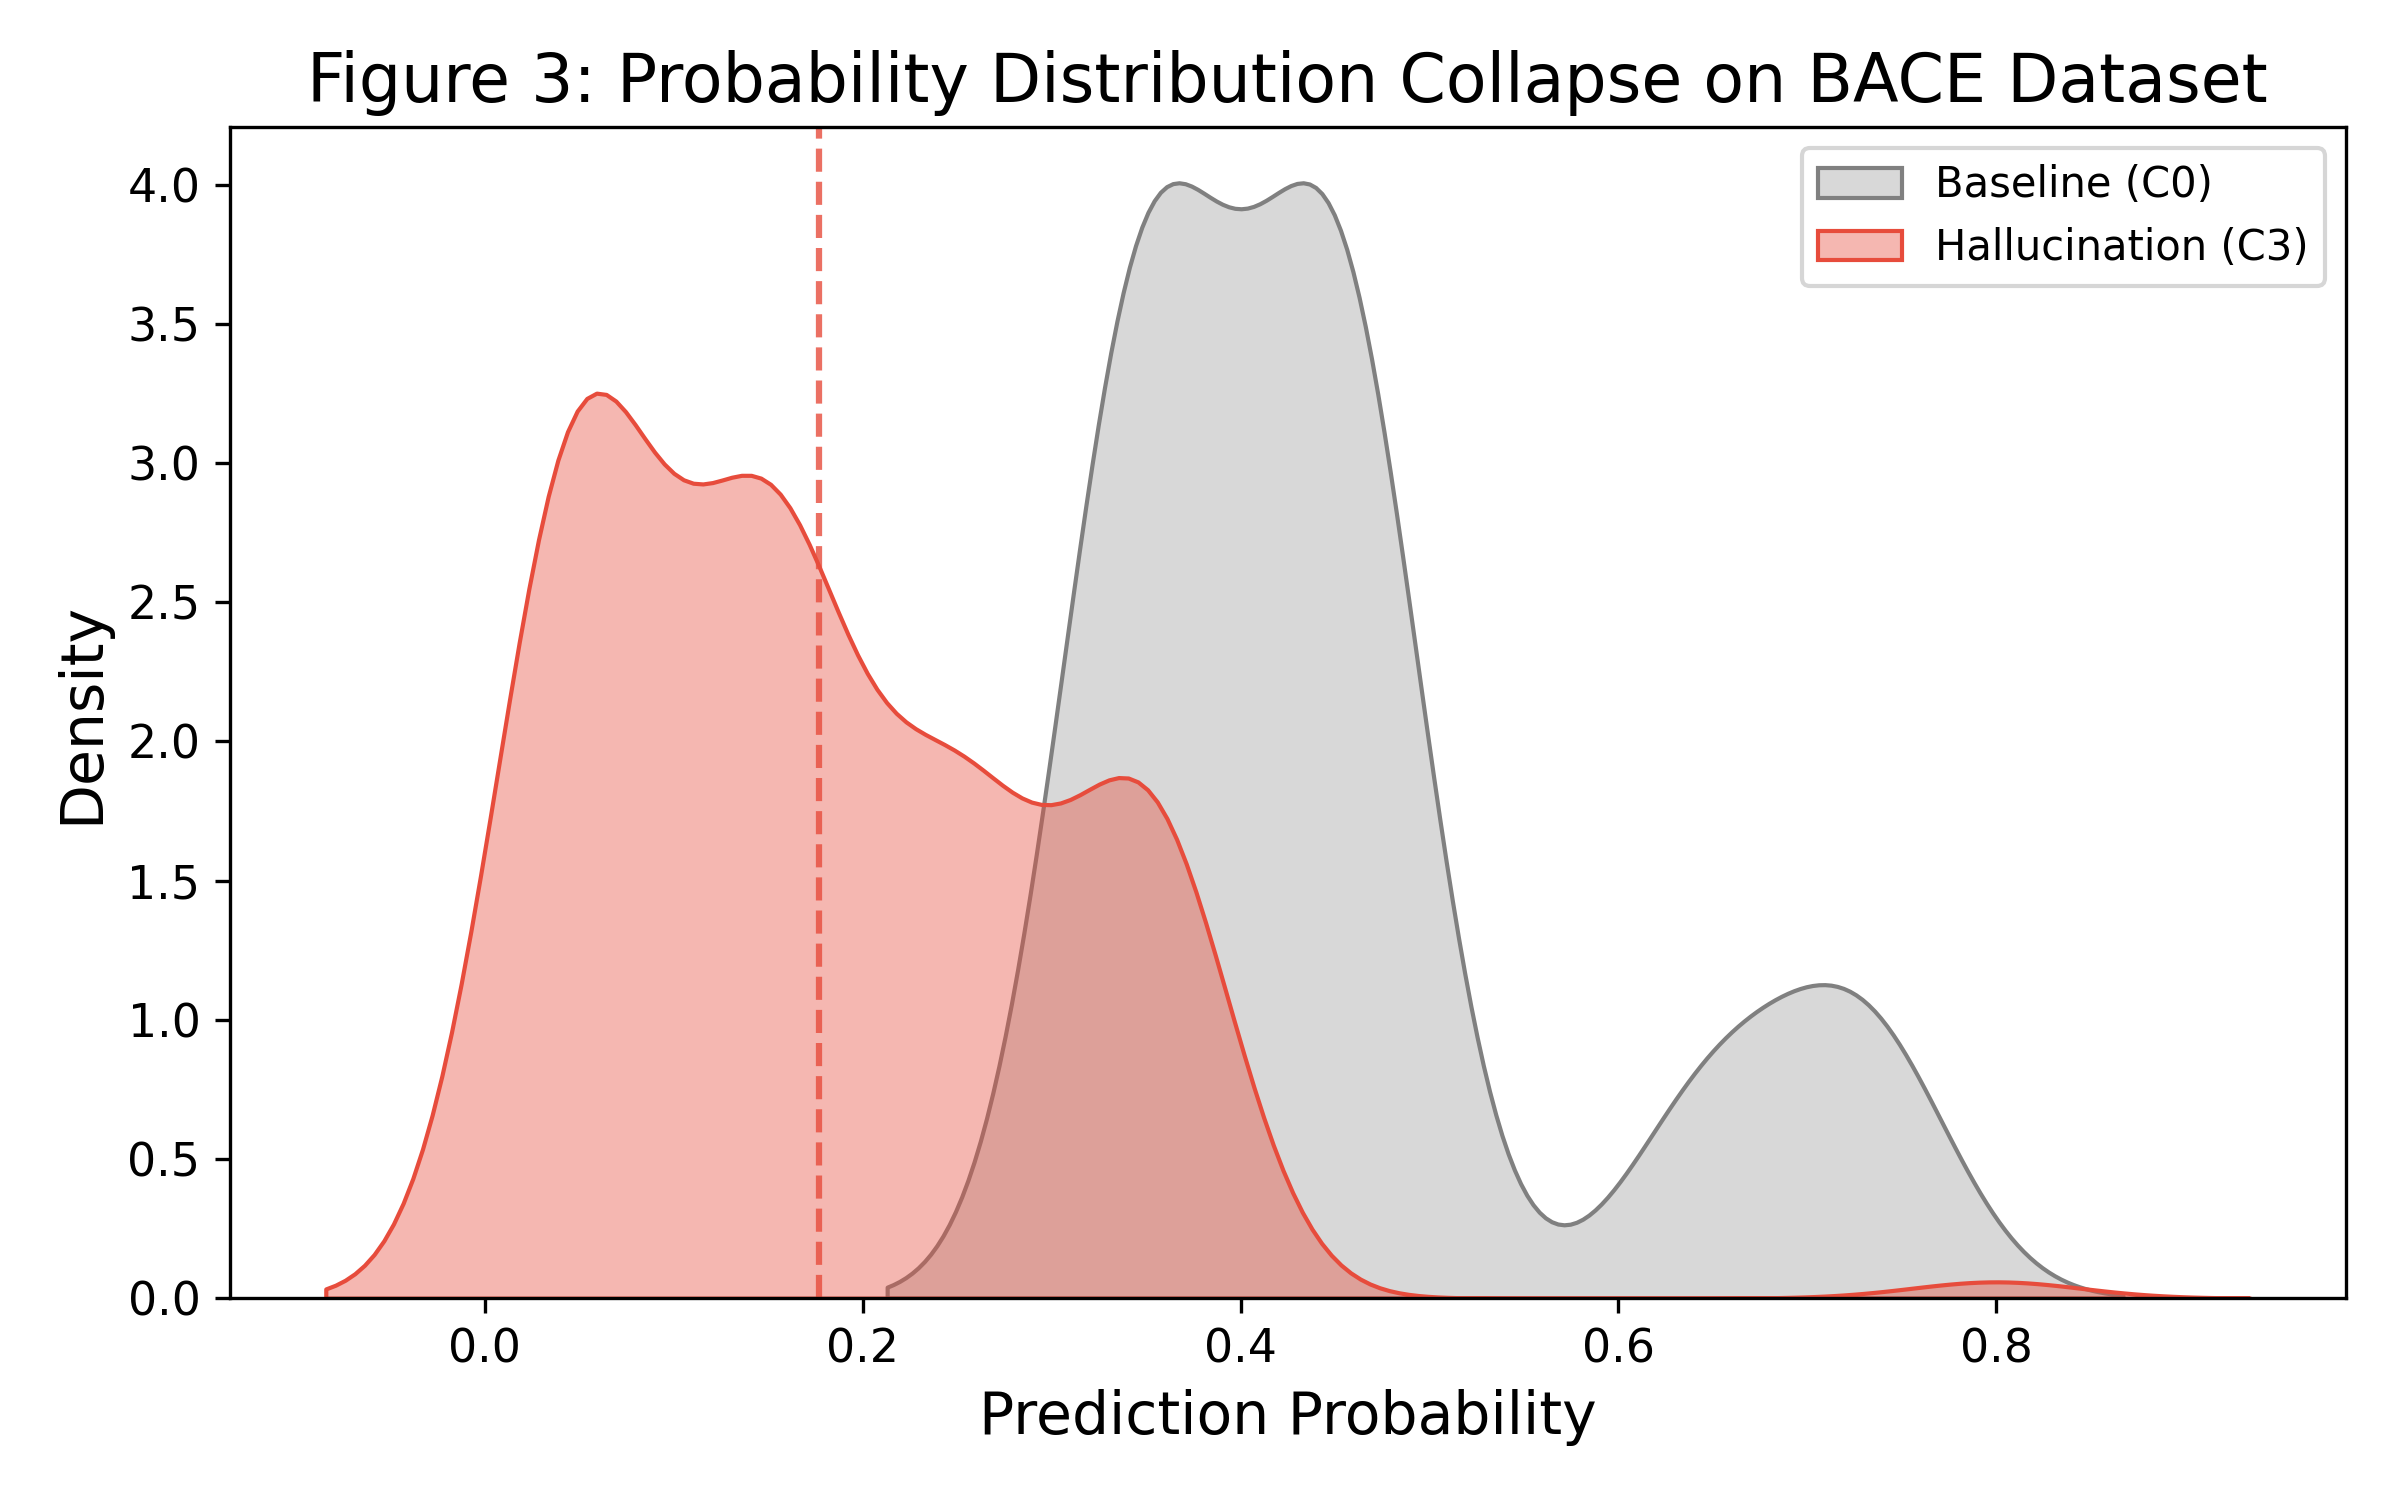
\includegraphics[width=\linewidth]{figures/figure3_negativity_collapse.png}
    \caption{Hallucination augmentation induces pronounced distributional compression on the BACE task, shifting the baseline bimodal prediction distribution toward a non-discriminative narrow peak near $p \approx 0.17$.}
    \label{fig:negativity}
\end{figure}

\subsection{Distribution of Hallucination Types}
Analysis of 356 naturally generated hallucinations across both datasets revealed a consistent distributional bias (Figure~\ref{fig:taxonomy}). Contextual Confabulation (CC) was the dominant category, accounting for approximately 80\% of all generated descriptions ($n=163$ of 204 for BBBP). Structural Phantom (SP) was the rarest category at 2.4\% ($n=5$ of 204 for BBBP). Despite this low natural frequency, forced SP hallucinations (C4a) exhibited the strongest predictive association on BBBP.

\begin{figure}[t]
    \centering
    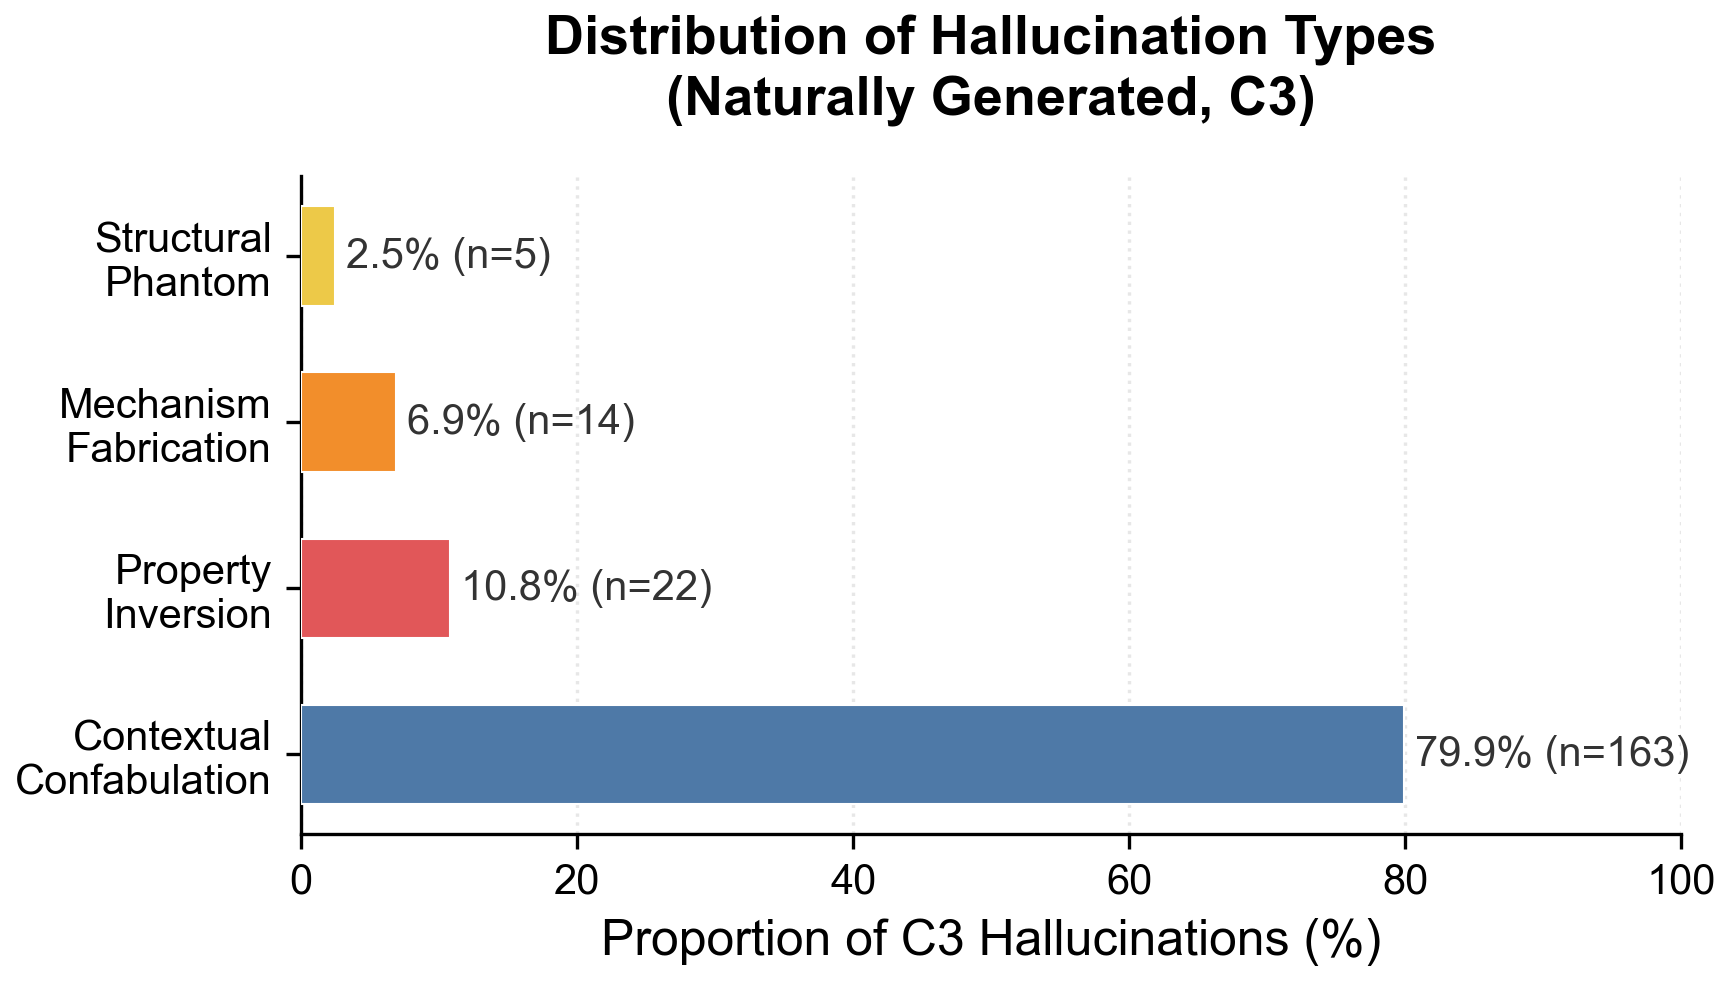
\includegraphics[width=0.8\linewidth]{figures/figure4_taxonomy_distribution.png}
    \caption{Free hallucinations exhibit a pronounced distributional bias toward generic Contextual Confabulation (CC), with structurally grounded perturbations (SP) occurring rarely despite their stronger association with predictive performance.}
    \label{fig:taxonomy}
\end{figure}
